\documentclass[xcolor=dvipsnames,split]{beamer}
% bibstuffs:
\usepackage[sort&compress]{natbib}
\bibliographystyle{apsr}
\bibpunct[:]{(}{)}{;}{a}{,}{,}

%\usepackage[all]{xy}
%\input xy
%\xyoption {all}




\usepackage{beamerthemesplit}
%\usecolortheme[rgb={0,0,.611764706}]{structure}
\definecolor{DukeBlue}{rgb}{0,0,.611764706}
\setbeamertemplate{items}[ball]
%\usetheme[height=11mm]{Rochester}
\usetheme[]{Boadilla} 

\definecolor{WUSTLgreen} {RGB} {44, 80, 54}
\definecolor{WUSTLred} {RGB} {149, 1, 1}
\definecolor{WUSTLtan} {RGB} {229, 210, 184}
\setbeamercolor{structure}{fg=WUSTLred, bg=WUSTLgreen}
\setbeamercolor{normaltext}{bg=black, fg=WUSTLtan}
\setbeamercolor{block title}{fg=WUSTLred}
\setbeamercolor{block title example}{fg=WUSTLgreen}
\setbeamercolor{frametitle}{fg=DukeBlue}
\setbeamercolor{title}{fg=DukeBlue}



\setbeamertemplate{blocks}[rounded]


\usepackage{rotating,amssymb,subfigure,tabularx}
\usepackage{caption}
\usepackage{graphicx}
\usepackage{color}
\usepackage{multicol}
\usepackage{array}
\usepackage{dcolumn}
\usepackage{multirow}
\usepackage{booktabs}
\usepackage{caption}
\setbeamerfont{tablefont}{size=\tiny}
\setbeamerfont{quotefont}{size=\small}


\newcommand{\bframe}{\begin{frame}}
\newcommand{\jacob}{\end{frame}}
\newcommand{\bi}{\begin{itemize}}
\newcommand{\ei}{\end{itemize}}
\newcommand{\be}{\begin{enumerate}}
\newcommand{\ee}{\end{enumerate}}
\newcommand{\vp}{\vspace{.5cm}}
\newcommand{\bis}{\begin{itemize}[<+->]}
\newcommand{\bes}{\begin{enumerate}[<+->]}
\newcommand{\red}[1]{\color{WUSTLred}{#1}}
\newcommand{\bc}{\begin{center}}
\newcommand{\ec}{\end{center}}
\newcommand{\eb}{\end{block}}
\newcommand{\ds}{\displaystyle}



\author[J. Montgomery, F. Hollenbach, M. Ward~~~~] 
{Jacob M. Montgomery  \inst{1} \and Florian M. Hollenbach  \inst{2} \and Michael D. Ward \inst{2}}


\institute[] % (optional, but mostly needed)
{
  \inst{1}%
Department of Political Science\\
Washington University in St. Louis
  \and
  \inst{2}%
  Department of Political Science\\
  Duke University}

 
\title[APSA, New Orleans, LA]{\textsc{Say Yes to the Guess: \\ Tailoring Elegant Ensembles on a Tight
  (Data) Budget}}


\date{August 31, 2012}


\begin{document}


\frame{\titlepage}


\section{Introduction}

\frame{\frametitle{Ensemble Bayesian Model Averaging (EBMA)}
EBMA is principled way of combining predictions to increase
out-of-sample performance
\begin{itemize}
\item Models are weighted based on calibration period
\item EBMA is a finite mixture model
\end{itemize}

\pause
\vp

\begin{block}{Predictive EBMA PDF}
$$p(y|f_{1}^{t^\ast}, \ldots, f_{K}^{t^\ast})=\overset{K}{\underset{k=1}{\sum}} w_k g_k(y|f_{k}^{t^*})$$
\end{block}
}

\frame{
\frametitle{Ensemble Bayesian Model Averaging (EBMA)}

\bis
\item$w_k$ estimated using EM algorithm
\item Increased weight given for
\bi
\item Accuracy
\item Uniqueness
\ei
\end{itemize}

}


\section{EBMA Adjustment}


\frame{\frametitle{Adjusting EBMA to Forecasting in the Social Sciences}     
Forecasting efforts in the social sciences are often hampered by data problems
\begin{itemize}
\item Missingness
\item Non-random missingness
\item Many forecasts, few observations
\end{itemize}
}



\frame{\frametitle{Predicting the Incumbent Voteshare in the 2012 Presidential Election}     

\begin{center}
\begin{footnotesize}
\begin{tabular}{rlrrrrrrrrr}
\toprule
  & F & A & C & H & LBRT & L & Hol & EW & Cuz \\ 
\midrule
  1992 & 55.7 & 46.3 & 49.7 & 48.9 & 47.3 &  &  &  &  \\ 
  1996 & 49.5 & 57.0 & 55.5 & 53.5 & 53.3 &  & 57.2 & 55.6 &  \\ 
  2000 & 50.8 & 53.2 & 52.8 & 54.8 & 55.4 & 60.3 & 60.3 & 55.2 &  \\ 
  2004 & 57.5 & 53.7 & 52.8 & 53.2 & 49.9 & 57.6 & 55.8 & 52.9 & 51.1 \\ 
  2008 & 48.1 & 45.7 & 52.7 & 48.5 & 43.4 & 41.8 & 44.3 & 47.8 & 48.1 \\ 
\bottomrule
\end{tabular}
\end{footnotesize}
\end{center}


}


\frame{\frametitle{Adjusting EBMA to Forecasting in the Social Sciences}     

Our solutions so far:
\bis
\item Fraley, Rafery and Gneiting (2010) approach to
  missing data
\item Introduce a ``wisdom of the crowds'' tuning parameter $c \in [0,1]$ 
\item A minimum ($\frac{c}{k}$) probability that each the observation
  is ``best'' predicted by each $k$ model. 
\end{itemize}

}

\section{Applications}

\frame{\frametitle{Predicting Quarterly Unemployment in the US}     

\begin{itemize}
\item Predictions from the Survey of Professional Forecasters (SPF) 
\item Green Book of the Fed
\item Predictions four quarters into the future
\item Rolling calibration window of ten quarters
\item Minimum of five forecasts in the calibration period for model inclusion
\end{itemize}
}

\frame{\frametitle{Observed and forecasted U.S. unemployment (1981-2007) }
\begin{center}
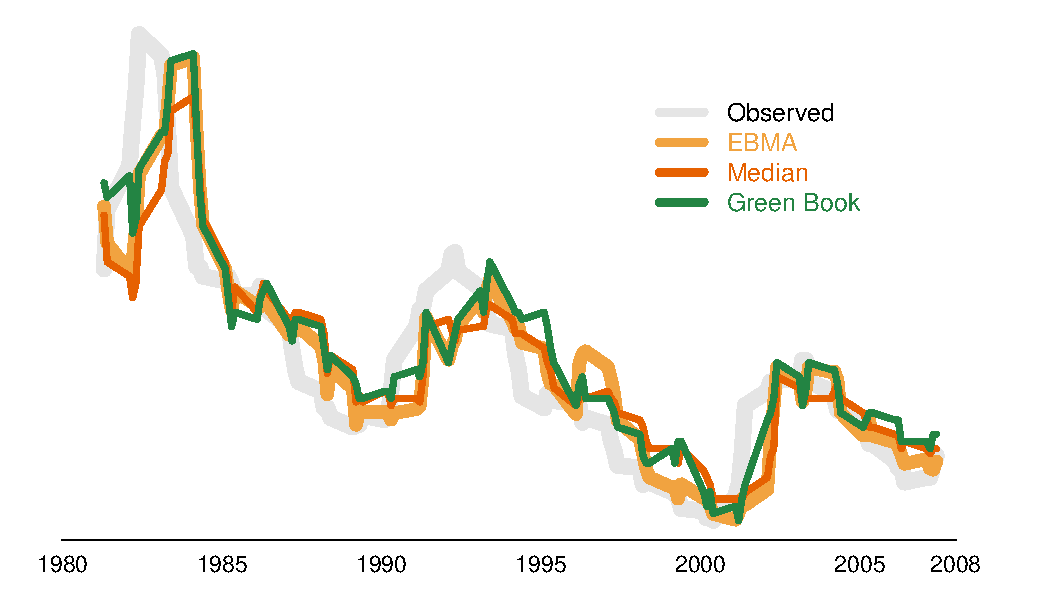
\includegraphics[scale=.65]{mdwtimeSeries2}
\end{center}

}


\frame{\frametitle{Comparing Forecasts of U.S. Unemployment}     
\begin{center}
\begin{footnotesize}
\begin{tabular}{lrrrrrrrr}
\toprule
 & MAE & RMSE & MAD & RMSLE & MAPE & MEAPE & MRAE & PW \\ 
\midrule
c=0& 0.54 & 0.74 & 0.37 & 0.093 & 8.37 & 6.49 & \textbf{0.73} & \textbf{27.36} \\ 
c=0.05& \textbf{0.54} & 0.74 &\textbf{ 0.37} & \textbf{0.093} & \textbf{8.33} & \textbf{6.30} & 0.75 & \textbf{27.36} \\ 
c=0.1& 0.54 & 0.74 & 0.35 & 0.093 & 8.40 & 6.44 & 0.76 & 28.30 \\ 
c=1 & 0.61 & 0.80 & 0.46 & 0.102 & 9.72 & 8.92 & 0.95 & 46.23 \\ 
GB & 0.57 & \textbf{0.73} & 0.43 & 0.093 & 9.37 & 8.81 & 1.00 & 45.28 \\ 
Median& 0.62 & 0.81 & 0.47 & 0.103 & 9.83 & 8.87 & 0.98 & 47.17 \\ 
Mean& 0.61 & 0.80 & 0.46 & 0.102 & 9.71 & 9.06 & 0.93 & 46.23 \\ 
\bottomrule
\end{tabular}
\end{footnotesize}
\end{center}
}



\frame{\frametitle{Predicting the Incumbent Voteshare in the 2012 Presidential Election}     

\begin{center}
\begin{footnotesize}
\begin{tabular}{rlrrrrrrrrr}
\toprule
  & F & A & C & H & LBRT & L & Hol & EW & Cuz \\ 
\midrule
  1992 & 55.7 & 46.3 & 49.7 & 48.9 & 47.3 &  &  &  &  \\ 
  1996 & 49.5 & 57.0 & 55.5 & 53.5 & 53.3 &  & 57.2 & 55.6 &  \\ 
  2000 & 50.8 & 53.2 & 52.8 & 54.8 & 55.4 & 60.3 & 60.3 & 55.2 &  \\ 
  2004 & 57.5 & 53.7 & 52.8 & 53.2 & 49.9 & 57.6 & 55.8 & 52.9 & 51.1 \\ 
  2008 & 48.1 & 45.7 & 52.7 & 48.5 & 43.4 & 41.8 & 44.3 & 47.8 & 48.1 \\ 
\bottomrule
\end{tabular}
\end{footnotesize}
\end{center}


}




\frame{\frametitle{Model weights and in-sample fit statistics for EBMA model of U.S. Presidential Elections (1992-2008)}
\begin{center}
\begin{footnotesize}
\begin{tabular}{lrrrr}
\toprule
 & \shortstack{EBMA\\ Weight}&RMSE &MAE \\ 
\midrule
EBMA &  & 1.92 & 1.56 \\ 
  Fair & 0.02 & 5.53 & 4.58 \\ 
  Abramowitz & 0.78 & 2.02 & 1.72 \\ 
  Campbell  & 0.07 & 3.46 & 2.88 \\ 
  Hibbs  & 0.04 & 2.68 & 2.44 \\ 
  Lewis-Beck, Rice, and Tien & 0.06 & 2.78 & 2.28 \\ 
  Lockerbie  & 0.00 & 7.33 & 6.97 \\ 
 Holbrook & 0.01 & 5.73 & 4.77 \\ 
  Erikson and Wlezien & 0.02 & 2.74 & 2.25 \\ 
  Cuz\`an & 0.00 & 1.27 & 0.95 \\ 
\bottomrule
\end{tabular}
\end{footnotesize}
\end{center}
}

\frame{\frametitle{Predictive Ensemble PDFs of Incumbent-Party Vote Share}
\begin{center}
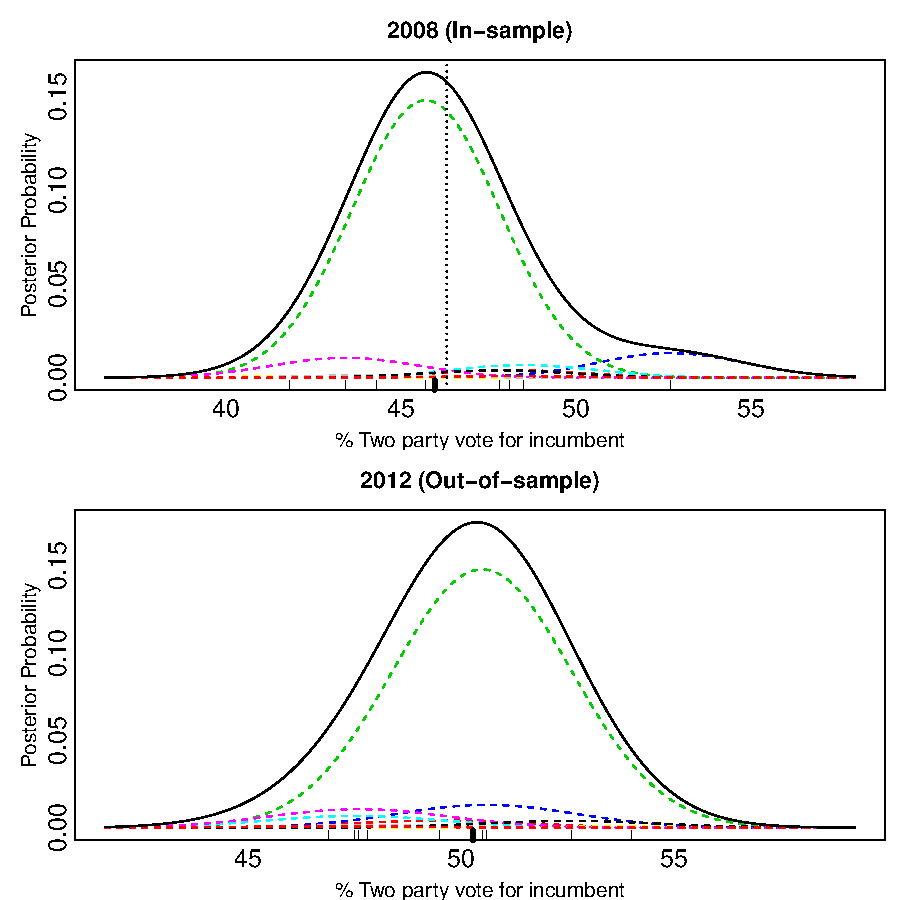
\includegraphics[scale=.5]{presForecast}
\end{center}

}



\section{Conclusion}
\frame{\frametitle{Future Work}     

\bis
\item Simulation study to show over-fitting problem
\item Alternative methods for handling missing forecasts
\item Estimate $c$ parameter
\end{itemize}

}

\end{document}\bye

